\chapter{State of the art}\label{C:State-Art}
This chapter briefly sketches out the state of the art of the embedded operating systems and its capabilities.

\section{Embedded Systems}\label{S:SOTA-Embedded-Systems}
Embedded Systems nowadays are taking relevance again with the Internet of Things, environment sensing, Wireless Sensor Networks and all new coming technologies that require low power consumption, small size, mobility environments, etc.
\\
\\
In Embedded Systems or Resource Constrained Systems it is interesting to take a look into the Hardware platform and its capabilities, the differences between platforms, and also which tools or unique features they offer to developers.
\\
\\
An operating system (OS) offers an interface with the hardware to make it independent from the applications that the device runs, making easy the interactions between hardware and the programs running on the machine.
\\
Until now, most embedded devices did not make use of operating systems and they where totally oriented to the designated application but as it has been explained in the introduction, the cost reduction in the production of systems has helped to increase the capacities so now is not unusual to embed a Linux system to simplify the manage of the resources.
\\
An OS is an important software that makes easy to develop applications, but it is important to maintain the features that the processor offers, avoiding performance or capabilities degradation. 
This bachelor thesis is focused on constrained-resource devices, where the processing capabilities and memory resources are limited, is fundamental to respect the above criteria.

\subsection{Operating Systems Architectures}\label{SOTA-Operating-Systems-Architectures}
In general, there are three types of operating system architectures for embedded devices, which are based on how applications are executed or included into the OS.

\begin{itemize}
\item \textbf{Monolithic:} The OS and the applications are combined into a single program. Normally in this situations the embedded device runs in the same process the OS and the program written to it. This type of architecture makes difficult to include new functions without rewriting much of the code.

\item \textbf{Modular:} The OS is running as a standalone program in the processor and has the ability of loading programs as modules. In terms of the development, it's possible to develop applications without writing in the core of the OS. Normally using modules developers can expand the capabilities of its software.

\item \textbf{Virtual-Machine:} The virtual machine creates an abstraction layer of its underlying hardware. This abstracted layer is common in every device that implements that virtual-machine. Using this type of operating system provides a helpful tool to achieve the well known slogan \textit{write once, run anywhere}. Although using virtual-machine devices simplifies the development on multiple devices, the performance of the platform normally will be reduced and in Real Time environments it isn't recommended to use it. It is interesting to remark that embedded virtual machines, differently from VMs in desktop or server environments, run on the bare metal so they also act as an operating system.
\end{itemize}

\subsection{Embedded Operating Systems}\label{SOTA-Embedded-Operating-Systems}
There is a wide range of Embedded Operating Systems each of them has strengths and weaknesses. Below different OS are described and compared.
 
\begin{itemize}
\item \textbf{TinyOS} is a popular open source OS for wireless constrained devices, many of them used in wireless sensor networks. It provides software abstractions from the underlying hardware. It is focused on wireless communications offering stacks for 6LoWPAN and ZigBee. It also supports secure networking and implements a \gls{RPL} taking in mind the forthcoming routing protocol for low power and lossy networks.
\\
However, TinyOS changes how programs should be developed, it intended to use non-blocking programming which means that it isn't prepared for long processing functions. For example, when TinyOS called to send a message the function will return immediately and after a while the send will be processed and then, TinyOS will make a callback to a function, for example \verb!send()!'s callback will be \verb!sendDone()!.

\item \textbf{FreeRTOS} is a free real-time OS that supports over 34 architectures and it is being developed by professionals under strict quality controls and robustness. It is used from toys to aircraft navigation and it is interesting for its real-time qualities. It has a very small memory footprint (RAM usage) and very fast execution, based on hard real-time interruptions performed by queues and semaphores. Apart from this, there are not constraints on the maximum number of tasks neither the priority levels that can be used on tasks. 

\item \textbf{Contiki} is similar to TinyOS in terms of portability between platforms and its code is open source. It also offers features similar to standard operating systems like threading, timers, file system and command line shell and uses modular architecture, loading or unloading programs from its kernel. Contiki is built on top of the Internet Standards supporting IPv4 and IPv6 and also the new low-power internet protocols which includes 6LoWPAN, RPL and CoAP.
\\
Contiki uses protothreads, which are designed for event-driven systems running on top of constrained devices, which is the case of Contiki's kernel. It provides blocking without having a real multi-threading system or a stack-switching.

\item \textbf{Micro Framework .NET} is a solution provided by Microsoft for resource-constrained devices which cannot execute the full .NET stack. It is Virtual-Machine based operating system that has a small implementation of the CLR making available to execute a small set of .NET classes. Its memory footprint is about 300KB and supports the common embedded peripherals like EEPROM, GPIO, SPI, UART, USB, ...
\\
One of its interesting features is that it offers the advantages of .NET language using Visual Studio and it also offers real-time debugging directly on the device.
\end{itemize}

\section{Micro Framework .NET}\label{S:SOTA-NETMF}
Micro Framework, also known as NETMF, has its roots in a project called \textbf{Smart Personal Objects Technology (SPOT)}. The first devices implementing the SPOT technology were smart-watches from Fossil and Suunto in 2004, but after them, some other devices also made use of SPOT, like kettles, weather stations and even map updates in Garmin devices. Microsoft wanted to create a technology for everyday devices, so they launched together with SPOT the MSN Direct, which was a set of network services capable of delivering information to the SPOT devices using FM radio broadcast signals.
\\
In 2008 the production of SPOT watches was discontinued, and in 2009 Microsoft released the source code of Micro Framework under Apache 2.0 license, making availably to the community, and shortly after this release the MSN Direct services where ceased.
\begin{figure}[H]\begin{center}
 \centering
  \captionsetup{justification=centering}
 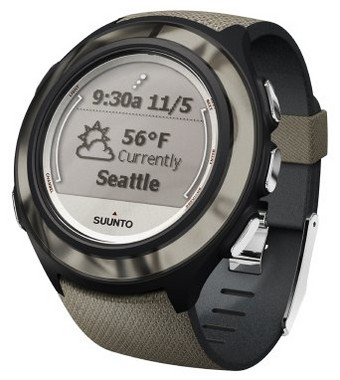
\includegraphics[scale=1]{pictures/stateoftheart/spot}
  \caption{SPOT watch \label{fig:State-Art-SPOT-Watch}}
\end{center}\end{figure}

\subsection{Devices using Micro Framework}\label{SS:SOTA-MicroFramework-Devices}
Since Microsoft released the Micro Framework source code, different companies had created different devices supporting .NET code and this stack.
\\
There are two major vendors producing chips and development kits for this software. Secret Labs produces the netduino family, which consists of the standard netduino, a netduino plus which is an enriched version. This one has better processor and memory, it includes an ethernet port and uses micro sd cards to provide storage. One of the interesting things of this two boards is that the layout is compatible with the arduino shields.
Secret Labs has another board called netduino go, which is similar to netduino plus but without storage and ethernet, and it does not use the typical arduino layout, so a globus module is required to use arduino shields. They also have another board called netduino mini whose size is similar to a rubber.
\\
GHI Electronics is another hardware manufacturer that has designed and released different boards implementing Micro Framework or modules for which its target platform is Micro Framework. GHI has a very wide range of products, for example FEZ Cerbuino Bee and FEZ Cerbuino NET, which are similar to the netduino plus in terms of performance. An interesting thing of FEZ devices over netduino is the possibility of loading native code (C/Assembly) for real-time requirements. For example HomeSense could run its Mesh driver in C and perform better than it performs using C\#.
\\
\\
In addition to the mentioned manufacturers, Microsoft Research in Cambridge has defined a hardware reference platform called .NET Gadgeteer, which defines how boards and modules must be in order to allow rapid prototyping of projects. Gadgeteer boards and modules share the same layout and connector schemes and are open to any company that wants to build products using those schematics.
\begin{figure}[H]\begin{center}
 \centering
  \captionsetup{justification=centering}
  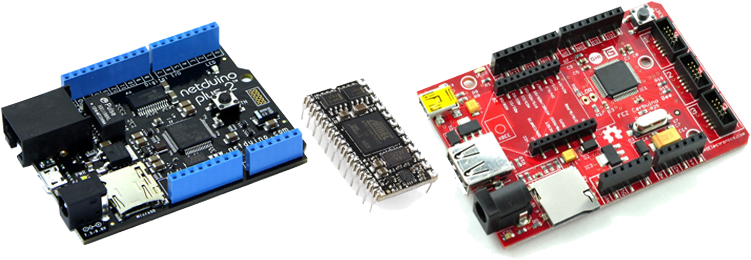
\includegraphics[width=0.8\textwidth]{pictures/stateoftheart/devices}
  \caption{Micro Framework devices. Netduino Plus on the left, Netduino Mini on the center and Cerbuino on the right.\label{fig:State-Art-NETMF-Boards}}
\end{center}\end{figure}

\subsection{NETMF on Linux}\label{SS:SOTA-NETMF-Linux}
After doing some research about implementations of Micro Framework on other devices, or running on top of other operating systems such as Linux, it was found a project that is currently porting NETMF to Linux, but for a very specific device called Eddy. This is a complete port of the virtual Machine so it has the original CLR interpreter and some of the functions working.
\\
Eddy is an ARM embedded device board that uses Linux. The port named above has been made as a demonstration of writing NETMF applications using a port on top of other operating systems. One of the majors problems of this port is that some drivers are not working at all, for example UART, SPI and \gls{I2C} which are 3 I/O protocols and ports used in HomeSense.
\\
Although this port is for the Eddy board, it can be ported to other devices using the appropriate cross-toolchain. Anyway it seems that there is a lack of possibilities to run Micro Framework code in other devices or operating systems.

\subsection{NETMF on RaspberryPi}\label{SS:SOTA-NETMF-RPI}
If it is hard to find an implementation of NETMF in Linux, it will be harder to find an implementation for Raspberry Pi. In other words, people in GHI forums are asking for NETMF ports for the Raspberry Pi but no one exists. At time of writing this thesis, a small port was uploaded to Codeplex \url{http://raspberrypinetmf.codeplex.com/} and uses the bcm2835 library to implement the Micro Framework functions.
\\
Leaving aside the NETMF implementations for the Raspberry Pi, a search on existing libraries to control the features of the board was done. There are existing libraries for many languages including C and C++, Python, Java, Ruby and .NET. The interesting ones are the C and .NET implementations, the first one because can be used in conjunction with .NET code via Platform Invocation Services. The second one is interesting for how has been done the implementation of the bcm2835 in this language, but after analysing it the conclusion was that there is a lack of libraries written in .NET.

\section{Conclusions}\label{S:SOTA-Conclusions}
There is not any real implementation of .NET Micro Framework for Linux. If IOSharp succeeds on implementing a library with the same methods of the framework it will become the first library to execute Micro Framework programs on any standard computer that runs Linux. In other words, this library will make easier the interaction between .NET programs and the underlying hardware.